\section{数值协议与局部输运证据}
\label{sec:numerical}

数值比较明确区分物理向量场、有限阶 Birkhoff 表示以及该表示的数值积分。
所有数值均取自已有冻结输出；制图没有执行新的物理仿真或训练。
共同降阶模型包含12个配置坐标、24个相空间坐标、20个几何单元及配置相关质量矩阵。
完整线圈计算采用12个圆线圈，每圈256个导线求积点。
$z=(Q,P)$ 为缩放正则坐标，$\tau=\omega_0t$，其中
$\omega_0=4.4576294085\,\mathrm{s}^{-1}$。
因此共同时间窗 $T=5\times10^{-4}$ 仅对应 $0.112167$\,ms。
下文状态误差为无量纲欧氏范数，并非毫米单位的末端误差。
能量和功率分别乘 $E_0=3.62\times10^{-7}$\,J 与 $E_0\omega_0$ 转换为 SI 单位。

\subsection{接受的数据来源与比较指标}

最终接受的输运运行名为 \texttt{inverse\_verified}。
高阶求导采用代数等价的完整 $M(Q)$ 逆，并在每个状态重算；物理场和原场参考仍保留原线性求解实现。
独立纯反向求导、有限差分及原生系数比较支持本次具体计算。
早期嵌套前向/反向求解结果，包括 \texttt{synthetic/main.json}，
不作为有效高阶导数证据，原文件继续归档。
程序成功结束本身不能验证导数正确性。
完整线圈范数求导失败及内存失败也保留其原始身份。

对步数 $N\in\{4,8,16\}$、$\eta=T/N$，定义
\begin{equation}
 \begin{aligned}
 E_f(\eta)&=\max_{0\leq j\leq N}\|z_j-z_f(\tau_j)\|_2,\\
 E_a(\eta)&=\max_{0\leq j\leq N}\|z_j-z_a(\tau_j)\|_2.
 \end{aligned}
 \label{eq:numerical-errors}
\end{equation}
其中 $z_f$、$z_a$ 分别为原场与表示场的独立 DOP853 参考。
连续表示误差在65个共同时间点计算。
积分观测阶为 $\log_2[E_a(2\eta)/E_a(\eta)]$；中心场差 $\|f_a-f\|_2$
另作时间喷流诊断。这些最大值均为采样量。
误差范数不能直接标量相加，向量误差抵消可能使 $E_f$ 小于 $E_a$。

合成原场和表示场的两组参考采用
$(\mathrm{rtol},\mathrm{atol},\eta_{\max})=(2\times10^{-10},2\times10^{-12},T/4)$
与 $(5\times10^{-12},5\times10^{-14},T/8)$。
完整线圈输运共享直接积分实验保存的共点分支参考。
后续独立桥接使用当前线圈核重新积分，在65个参考状态上的最大差为 $5.77\times10^{-19}$。
重新拟合偏置电流的最大差为 $6.56\times10^{-14}$\,A，故这里是共同数学反馈定义下，
已量化舍入差的比较，不宣称拟合电流逐位相同。

\subsection{输运阶、积分阶与成本}

合成载荷光滑、状态相关且非比例，不是血流或接触标定模型。
其三阶以内一形式系数的空间次数为 $(2,2,1)$；
完整线圈共点载荷二阶以内的空间次数为 $(2,1)$。
只有这些系数多项式被缓存：原 Hamiltonian、向量场、Jacobian 和完整质量矩阵均在当前状态计算。
两个展开均固定时间原点和缓存中心。

图~\ref{fig:transport} 区分更高输运阶与二阶图中点积分。
在 $\tau=T$，合成分支中心场误差依次为
$3.6233\times10^{-5}$、$6.4510\times10^{-6}$、$1.3243\times10^{-6}$；
连续轨迹差依次为 $8.8402\times10^{-9}$、$1.0556\times10^{-9}$、$1.6462\times10^{-10}$。
但16步原场误差为 $9.6995\times10^{-9}$、$2.0033\times10^{-9}$、$2.2615\times10^{-9}$，
故三阶在本次总误差比较中并非最好。
三个表示场积分的观测阶均约为 $1.9992$。

完整线圈反馈的连续差从 $5.0108\times10^{-8}$ 降至 $1.0785\times10^{-9}$，
最细原场误差从 $5.0169\times10^{-8}$ 降至 $2.4959\times10^{-9}$。
后者仍高于同一原场直接中点的 $2.2449\times10^{-9}$。
这里取得的是可计算的局部表示及其二形式，而不是原场精度全面占优或控制性能已经改善。

辅助 Moser 问题沿自身参数进行数值积分，并非机器人的精确流。
算法传播状态、时间及高阶敏感度，通过反向辅助积分获得逆图。
完整增量残差容差为 $2\times10^{-13}$。
合成分支和完整线圈分支记录的总墙钟时间分别为 $614.900$\,s 和 $1223.641$\,s，
包含系数构造与参考计算。
完整线圈每个网格运行耗时 $44.69$--$116.07$\,s，其中辅助图计算耗时 $0.60$--$1.38$\,s。
这些共享机器上的时间属于实测成本，不构成算法速度排名。

\begin{figure*}[t]
\centering
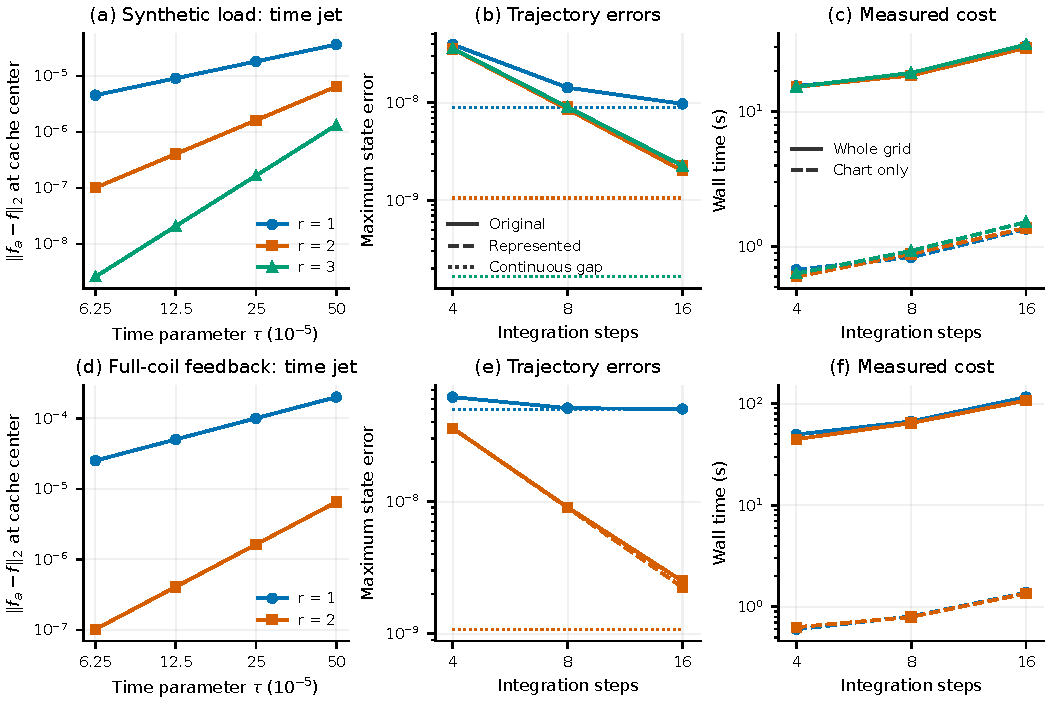
\includegraphics[width=\textwidth]{../figures/transport.pdf}
\caption{最终接受的输运计算。上下两行分别为合成载荷与完整线圈共点反馈。
左：固定缓存中心的原生时间喷流误差。
中：相对原场（实线）与表示场（虚线）的采样轨迹误差，点线为连续参考差；
不同输运阶的表示场误差曲线几乎重合。
右：完整网格墙钟时间与其中辅助图的耗时；系数构造和参考计算不计入这些逐网格时间。
颜色和标记区分输运阶，该阶数不改变中点的二阶时间离散。}
\label{fig:transport}
\end{figure*}

\subsection{直接积分器与失败域}

各直接积分分支分别使用自己的物理场与两组独立 DOP853 参考，设置为
$(2\times10^{-11},2\times10^{-13},T/4)$ 和 $(5\times10^{-13},5\times10^{-15},T/8)$。
固定电流、比例阻尼和共点反馈的参考细化差分别为
$1.24\times10^{-17}$、$8.01\times10^{-18}$、$1.38\times10^{-17}$。
所有方法均从规定的幅值 $0.01$ 初态出发，但只在同一分支内比较误差。
15个方法/网格组合及6组参考总耗时 $690.713$\,s。

固定电流保守分支中，中点与继承的非可分 Central4 最细误差分别为
$2.2449\times10^{-9}$ 和 $1.4749\times10^{-13}$，观测阶分别为 $1.9996$ 和 $3.9966$
（图~\ref{fig:integrators}）。
对合成比例阻尼 $-0.2P$，普通中点与加权中点均为二阶，
但仅加权构造以 $K(\tau)=e^{0.2\tau}K_0$ 为保持目标。
其最细缺陷为 $1.11\times10^{-15}$，普通中点则为 $1.17\times10^{-9}$。
真实共点电流律在未知中点求值，并使用完整反馈 Jacobian。
其正则二形式缺陷为 $3.93\times10^{-4}$：很小的积分残差并不意味着保持 $K_0$。
Central4 和比例加权格式没有被应用于这一一般反馈分支。
结构诊断对全部中点步骤采样理想隐式切映射，而 Central4 仅采样首步；
不宣称浮点程序是精确辛映射。

局部性另有显式测试。
25个时间参数图探测中，合成二阶在 $\tau=0.2$、三阶在 $0.05$ 和 $0.2$，
以及完整线圈二阶在 $0.2$ 时辅助路径越出声明半径 $0.002$，因而被拒绝。
另有两个域外输入按预期拒绝。
这些属于辅助图探测，并非长时间机器人轨迹。
多项式非退化界没有有向舍入，故不是区间证书。
证据支持短时间窗光滑场中的数值连接，尚未建立图间过渡、受限采样反馈结构、
长时间收敛或新的 KAM 证书。

\begin{figure*}[t]
\centering
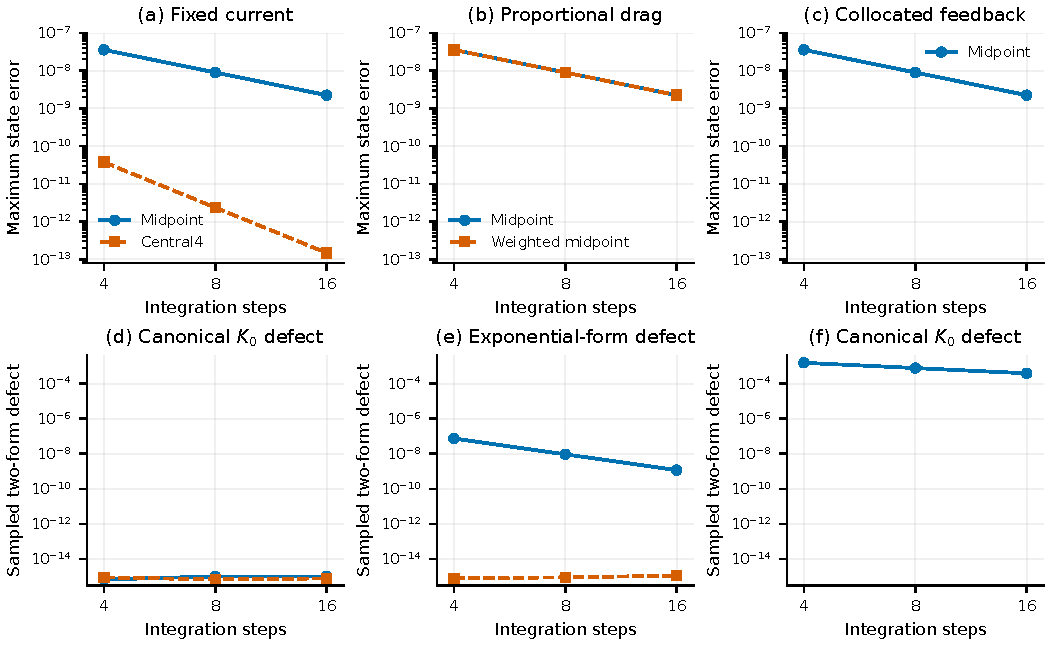
\includegraphics[width=\textwidth]{../figures/integrators.pdf}
\caption{分支内的直接积分比较。
上：相对各自分支精细参考的误差。
下：固定电流与共点反馈的正则二形式缺陷，以及比例阻尼的指数加权二形式缺陷。
比例分支两条误差曲线几乎重合。
缺陷基于理想隐式切映射采样，Central4 仅采样首步。
共点分支非零正则缺陷说明需要针对实际场构造表示，并不否定其二阶轨迹收敛。}
\label{fig:integrators}
\end{figure*}
